% AHCP data-descriptor article. Every result is a macro from numbers.tex or a table from tables/,
% both written by code/07_paper_stats.py. Build: pdflatex ahcp_article (twice).
\documentclass[10pt,twocolumn,letterpaper]{article}
\usepackage[T1]{fontenc}
\usepackage[utf8]{inputenc}
\usepackage{utopia}
\usepackage[letterpaper,left=0.68in,right=0.68in,top=0.85in,bottom=0.9in,columnsep=0.22in,headsep=0.3in]{geometry}
\usepackage{amsmath,amssymb}
\usepackage{graphicx,booktabs,array,multirow,enumitem,xcolor,url}
\usepackage[font=footnotesize]{caption}
\usepackage{titlesec,fancyhdr,microtype,cite,stfloats,balance}
\usepackage{tikz}
\usetikzlibrary{positioning,arrows.meta,fit,calc}
\usepackage[hidelinks]{hyperref}
\newcommand{\SDateConflicts}{485}
\newcommand{\SDateConflictsOverOneDay}{85}
\newcommand{\SInspectionColumns}{25}
\newcommand{\SInspections}{313,732}
\newcommand{\SInspectionsMf}{212,695}
\newcommand{\SInspectionsPh}{101,037}
\newcommand{\SInspectionsTwentytenTwentytwelve}{28}
\newcommand{\SLegacyAnyCandidate}{5,213}
\newcommand{\SLegacyUniqueCandidate}{5,012}
\newcommand{\SLihtcFlagNLinkedPct}{5.45}
\newcommand{\SLihtcFlagYLinkedPct}{54.12}
\newcommand{\SLihtcLinked}{6,110}
\newcommand{\SLihtcLinkedAddress}{5,857}
\newcommand{\SLihtcLinkedProximity}{253}
\newcommand{\SMedianInspectionsPerProperty}{5}
\newcommand{\SNVintages}{9}
\newcommand{\SNspireHudFlag}{28,934}
\newcommand{\SNspireInferred}{0}
\newcommand{\SNspireMfBeforeStart}{149}
\newcommand{\SPlacesMatched}{58,803}
\newcommand{\SPlacesMatchedPct}{98.47}
\newcommand{\SPlacesTracts}{27,890}
\newcommand{\SProperties}{65,337}
\newcommand{\SPropertiesBothProtocols}{25,237}
\newcommand{\SPropertiesMf}{42,127}
\newcommand{\SPropertiesMultiInspection}{58,400}
\newcommand{\SPropertiesNoCoordinates}{5,609}
\newcommand{\SPropertiesPh}{23,210}
\newcommand{\SPropertiesPhAmp}{8,426}
\newcommand{\SPropertiesPhPreAmp}{14,784}
\newcommand{\SPropertyColumns}{68}
\newcommand{\SQaHardFails}{0}
\newcommand{\SRawRows}{445,664}
\newcommand{\SScoreConflicts}{367}
\newcommand{\SSnapshotRows}{445,664}
\newcommand{\SSubsidyLinked}{34,997}
\newcommand{\SSubsidyLinkedCurrentMfPct}{99.04}
\newcommand{\SSubsidyLinkedCurrentPhPct}{99.71}
\newcommand{\STractAssigned}{59,716}
\newcommand{\STractAssignedPct}{91.4}
\newcommand{\STractCountyAgreePct}{99.93}
\newcommand{\SUpcsHudFlag}{15,558}
\newcommand{\SUpcsInferred}{269,240}
\newcommand{\ctxFailHigh}{8.9}
\newcommand{\ctxFailLow}{2.4}
\newcommand{\ctxN}{20,565}
\newcommand{\ctxSpearman}{$-$0.18}
\newcommand{\curFailN}{1,503}
\newcommand{\curFailPct}{4.3}
\newcommand{\curMF}{28,787}
\newcommand{\curNspirePct}{78.4}
\newcommand{\curPH}{6,135}
\newcommand{\curPlacesPct}{98.44}
\newcommand{\curProps}{34,922}
\newcommand{\curTractPct}{99.99}
\newcommand{\curUnits}{3,332,158}
\newcommand{\curUnitsKnownPct}{99.1}
\newcommand{\dateConfMaxDays}{3,179}
\newcommand{\dateConfOneDay}{400}
\newcommand{\dateConfPctMulti}{0.55}
\newcommand{\exInspRows}{8}
\newcommand{\exSnapRows}{12}
\newcommand{\failMFNSPIREB}{4.4}
\newcommand{\failMFUPCSA}{9.2}
\newcommand{\failMFUPCSB}{4.6}
\newcommand{\failPHNSPIREB}{15.6}
\newcommand{\failPHUPCSA}{11.1}
\newcommand{\failPHUPCSB}{9.5}
\newcommand{\inspLegacy}{177,986}
\newcommand{\inspMaxVintages}{8}
\newcommand{\inspMultiVintage}{88,497}
\newcommand{\inspOneVintage}{225,235}
\newcommand{\inspPostLegacy}{135,746}
\newcommand{\inspPostOneVintage}{47,249}
\newcommand{\ivLongMFA}{10.9}
\newcommand{\ivLongMFB}{12.9}
\newcommand{\ivLongMFC}{70.4}
\newcommand{\ivLongMFG}{99.9}
\newcommand{\ivLongPHA}{2.5}
\newcommand{\ivLongPHB}{4.2}
\newcommand{\ivLongPHC}{60.9}
\newcommand{\ivLongPHG}{99.9}
\newcommand{\ivMedMFA}{2.01}
\newcommand{\ivMedMFB}{2.34}
\newcommand{\ivMedMFC}{4.61}
\newcommand{\ivMedMFG}{6.45}
\newcommand{\ivMedPHA}{1.71}
\newcommand{\ivMedPHB}{2.05}
\newcommand{\ivMedPHC}{4.14}
\newcommand{\ivMedPHG}{5.14}
\newcommand{\legacyAny}{5,213}
\newcommand{\legacyAnyPct}{35.3}
\newcommand{\legacyTotal}{14,784}
\newcommand{\legacyUnique}{5,012}
\newcommand{\lihtcFalse}{5.5}
\newcommand{\lihtcMulti}{522}
\newcommand{\lihtcNLinked}{815}
\newcommand{\lihtcNNot}{14,128}
\newcommand{\lihtcPPV}{64.7}
\newcommand{\lihtcRows}{50,566}
\newcommand{\lihtcSens}{54.1}
\newcommand{\lihtcYLinked}{1,491}
\newcommand{\lihtcYNot}{1,264}
\newcommand{\lqBlockGroupPct}{1.5}
\newcommand{\lqRooftopPct}{92.8}
\newcommand{\lqZipCentroidPct}{2.2}
\newcommand{\lqZipFourPct}{3.4}
\newcommand{\meanMFNSPIREB}{88.9}
\newcommand{\meanMFUPCSA}{81.5}
\newcommand{\meanMFUPCSB}{85.1}
\newcommand{\meanPHNSPIREB}{81.1}
\newcommand{\meanPHUPCSA}{80.4}
\newcommand{\meanPHUPCSB}{81.3}
\newcommand{\mfAssistedRows}{23,783}
\newcommand{\mfInsuredRows}{17,582}
\newcommand{\nCounties}{2,930}
\newcommand{\nPHA}{3,149}
\newcommand{\nStates}{55}
\newcommand{\nTracts}{28,250}
\newcommand{\nVintages}{9}
\newcommand{\nspireAtFiftyNine}{675}
\newcommand{\nspireFiftyFiveToFiftyNine}{3.1}
\newcommand{\nspirePctFiftyNine}{2.3}
\newcommand{\nspireSixtyToSixtyFour}{0.5}
\newcommand{\pctOneVintage}{71.8}
\newcommand{\pctPostOneVintage}{34.8}
\newcommand{\pctPropOneInsp}{10.6}
\newcommand{\phDevRows}{6,211}
\newcommand{\placesCT}{908}
\newcommand{\placesTractsAll}{83,522}
\newcommand{\propMaxInsp}{15}
\newcommand{\propMeanInsp}{4.80}
\newcommand{\propOneInsp}{6,937}
\newcommand{\propSpanMedianYears}{8.2}
\newcommand{\rawFiles}{18}
\newcommand{\rowsInspections}{313,732}
\newcommand{\rowsPhLegacyCrosswalk}{5,439}
\newcommand{\rowsProperties}{65,337}
\newcommand{\rowsSnapshots}{445,664}
\newcommand{\rowsTractHealth}{27,890}
\newcommand{\scoreConfCrossSixty}{72}
\newcommand{\scoreConfDown}{11}
\newcommand{\scoreConfMax}{55.0}
\newcommand{\scoreConfMedian}{8.0}
\newcommand{\scoreConfPctMulti}{0.41}
\newcommand{\scoreConfSame}{0}
\newcommand{\scoreConfUp}{356}
\newcommand{\trNNMFDelta}{12.0}
\newcommand{\trNNMFN}{1,060}
\newcommand{\trNNMFNewFail}{6.7}
\newcommand{\trNNMFR}{0.18}
\newcommand{\trNNPHDelta}{10.9}
\newcommand{\trNNPHN}{388}
\newcommand{\trNNPHNewFail}{8.2}
\newcommand{\trNNPHR}{0.27}
\newcommand{\trUNMFDelta}{2.1}
\newcommand{\trUNMFN}{20,746}
\newcommand{\trUNMFNewFail}{3.7}
\newcommand{\trUNMFR}{0.22}
\newcommand{\trUNPHDelta}{1.6}
\newcommand{\trUNPHN}{4,457}
\newcommand{\trUNPHNewFail}{11.0}
\newcommand{\trUNPHR}{0.32}
\newcommand{\trUNgapMedian}{5.42}
\newcommand{\trUUMFDelta}{0.5}
\newcommand{\trUUMFN}{52,094}
\newcommand{\trUUMFNewFail}{3.7}
\newcommand{\trUUMFR}{0.37}
\newcommand{\trUUPHDelta}{$-$1.8}
\newcommand{\trUUPHN}{15,717}
\newcommand{\trUUPHNewFail}{7.8}
\newcommand{\trUUPHR}{0.49}
\newcommand{\trUUgapMedian}{2.74}
\newcommand{\tractContains}{59,681}
\newcommand{\tractCountyAgree}{59,644}
\newcommand{\tractCountyN}{59,684}
\newcommand{\tractHudCompareN}{34,986}
\newcommand{\tractHudSameCode}{98.1}
\newcommand{\tractHudSameCounty}{99.97}
\newcommand{\tractNearest}{35}
\newcommand{\tractNoCoord}{5,609}
\newcommand{\tractOutside}{12}
\newcommand{\tractPolygons}{85,187}
\newcommand{\upcsAtFiftyNine}{0.4}
\newcommand{\upcsFiftyFiveToFiftyNine}{1.8}
\newcommand{\upcsSixtyToSixtyFour}{3.6}


% ---- journal-style layout ---------------------------------------------------------------------------------
\pagestyle{fancy}\fancyhf{}
\fancyhead[L]{\scriptsize PREPRINT, OCTOBER 2026}\fancyhead[R]{\scriptsize\thepage}
\renewcommand{\headrulewidth}{0pt}
\renewcommand{\thesection}{\Roman{section}}
\renewcommand{\thesubsection}{\thesection-\Alph{subsection}}
\titleformat{\section}{\centering\normalsize\scshape}{\thesection.}{0.5em}{}
\titleformat{\subsection}{\normalsize\itshape}{\Alph{subsection}.}{0.5em}{}
\titleformat{\subsubsection}[runin]{\normalsize\itshape}{\arabic{subsubsection})}{0.4em}{}[:]
\titlespacing*{\section}{0pt}{2.2ex plus .6ex minus .2ex}{1.1ex}
\titlespacing*{\subsection}{0pt}{1.8ex plus .5ex minus .2ex}{0.8ex}
\titlespacing*{\subsubsection}{\parindent}{1.0ex plus .3ex}{0.4em}
\renewcommand{\thetable}{\Roman{table}}
\captionsetup[table]{name=TABLE,labelsep=newline,textfont=sc,justification=centering,skip=4pt}
\captionsetup[figure]{name=Fig.,labelsep=period,justification=justified,singlelinecheck=false,skip=4pt}
\newcommand{\runhead}[1]{\par\vspace{0.35ex}\noindent\textbf{#1}\hspace{0.35em}}
\newcommand{\col}[1]{\texttt{\small #1}}
\newcommand{\appsection}[2]{\par\vspace{2.2ex}\begin{center}\textsc{Appendix #1}\\\textsc{#2}\end{center}\vspace{0.6ex}}
\setlength{\parskip}{0pt}\setlength{\parindent}{1em}
\setlist{leftmargin=1.6em,itemsep=0.25ex,topsep=0.5ex}
\renewcommand{\arraystretch}{1.05}
\sloppy\raggedbottom
\hyphenation{multi-family Zenodo}

\begin{document}
\twocolumn[
\begin{center}
{\fontsize{22}{26}\selectfont The Assisted Housing Condition Panel: Reconstructing Inspection Histories for HUD-Assisted Housing from Overwritten Public Score Files\par}
\vspace{1.2ex}
{\large Ayishatu Ameen\par}
\vspace{3.2ex}
\end{center}
]

\begingroup
\renewcommand{\thefootnote}{}
\footnotetext{A. Ameen is an independent researcher in Hartford, Connecticut, USA (e-mail: ameenayishatu4@gmail.com; ORCID: 0009-0009-9386-2526).}
\footnotetext{The dataset described here is archived at \url{https://doi.org/10.5281/zenodo.23200319}; the code is at \url{https://github.com/AYISHATUAMEEN/ahcp}. This work received no external funding.}
\endgroup

\noindent\textbf{\textit{Abstract}---The U.S. Department of Housing and Urban Development (HUD) publishes physical inspection scores for public housing and for assisted and insured multifamily housing as spreadsheets that are replaced over time and that, since 2016, list only each property's most recent inspection. The public record of how a property's condition changed is therefore lost with every refresh. We describe the Assisted Housing Condition Panel (AHCP) v1.0, which stacks the \nVintages{} score-file vintages HUD still publishes (\SRawRows{} rows in \rawFiles{} files, 2011 to 2026 vintages), harmonizes their schemas and identifiers, and reconstructs \SInspections{} unique inspections of \SProperties{} properties dated 2000 to 2026. Each inspection carries the protocol under which it was scored: HUD's own flag for \SNspireHudFlag{} inspections under the National Standards for the Physical Inspection of Real Estate (NSPIRE) and \SUpcsHudFlag{} under the Uniform Physical Condition Standards (UPCS), and a date-based inference for the remainder. Properties are linked to 2020 census tracts by point-in-polygon assignment (\STractAssignedPct\% of properties; county agreement \STractCountyAgreePct\%), to HUD subsidy records (\SSubsidyLinkedCurrentMfPct\% of multifamily and \SSubsidyLinkedCurrentPhPct\% of public housing properties in the 2026 vintage), to Low-Income Housing Tax Credit projects, and to tract-level health estimates. We document what the public files cannot recover: no vintage covers 2010 to 2012, and \pctPostOneVintage\% of inspections dated after that gap appear in only one vintage, so a superseded inspection is easily lost. Where vintages disagree about the same inspection (\SScoreConflicts{} scores), the later file is higher in \scoreConfUp{} cases. Score distributions differ by protocol, with \nspirePctFiftyNine\% of NSPIRE scores at exactly 59, the value assigned by the unit-threshold rule, so levels should not be compared across the 2023 changeover without adjustment. All tables, code, a codebook, and a hash-level provenance log are openly released.}

\vspace{1.0ex}
\noindent\textbf{\textit{Index Terms}---Housing quality, public housing, multifamily assisted housing, physical inspection, NSPIRE, UPCS, panel data, data harmonization, record linkage, open data.}

\section{Introduction}
Federal rental assistance in the United States is delivered largely through buildings: public housing owned by local agencies, and privately owned multifamily properties that carry project-based subsidies or mortgage insurance from HUD. The condition of those buildings is a determinant of residents' health and safety~\cite{krieger2002,jacobs2011,swope2019}, and it is the main thing HUD measures when it inspects them. Since the late 1990s HUD's Real Estate Assessment Center (REAC) has inspected each property on a recurring schedule and assigned a score from 0 to 100; properties scoring below 60 fail and face enforcement~\cite{cfr5g,gao2019}.

HUD releases these scores to the public~\cite{hudpis}. The release is a pair of spreadsheets, one for public housing and one for multifamily properties, posted at irregular intervals. Each new pair replaces the working view of the portfolio, and since the 2016 release each file holds one row per property: the latest inspection. A researcher who downloads the current file sees a cross-section. The earlier inspection of the same property, which may have been a failure that prompted the reinspection now shown, is not in it. Oversight bodies have repeatedly examined whether the inspection process identifies and resolves poor conditions~\cite{gao2001,gao2019,oig2024}; outside researchers who want to study the same question longitudinally start from files that were not designed to support it.

The older files have not been removed, however. HUD's page still links nine vintages, from a 2011 file holding full histories for 2000 to 2009 to the April 2026 file. Stacked, they recover much more than any one of them shows. They also disagree with one another in column names, column meanings, date encodings, identifier schemes, and occasionally in the score reported for the same inspection. In 2023 HUD replaced the inspection protocol itself, moving from the Uniform Physical Condition Standards (UPCS) to the National Standards for the Physical Inspection of Real Estate (NSPIRE)~\cite{nspirerule,nspirescoring}, so that the most recent scores are produced by a different scoring model than the earlier ones.

This article describes the Assisted Housing Condition Panel (AHCP) v1.0~\cite{ahcp}, an open dataset that performs this reconstruction once, documents every rule it applies, and measures what the result does and does not cover. Our contributions are:
\begin{itemize}
\item \textbf{A reconstructed inspection panel.} \SInspections{} unique inspections of \SProperties{} properties (\SInspectionsMf{} multifamily, \SInspectionsPh{} public housing inspections), keyed on stable identifiers, with a lossless snapshot table that maps every value back to a source file and row.
\item \textbf{Protocol flags with stated provenance.} Each inspection is labelled UPCS or NSPIRE, and each label records whether it is HUD's flag or an inference.
\item \textbf{Four linkages.} Census tract, HUD subsidy record, Low-Income Housing Tax Credit (LIHTC) project, and tract health estimates, each with a recorded match method and a measured match rate.
\item \textbf{A quantified account of censoring.} We measure the 2010 to 2012 gap, the share of inspections that survive in a single vintage, the turnover between vintages, and the resulting lengthening of observed inter-inspection intervals.
\item \textbf{Validation evidence.} Conservation and uniqueness checks, an independent round trip against the latest workbooks, cross-vintage reconciliation statistics, geocoding agreement with two independent references, and an assessment of the LIHTC link against HUD's own tax-credit indicator.
\end{itemize}
We do not claim that AHCP is a complete inspection history, that scores are comparable across protocols, or that the tax-credit and legacy-identifier links are confirmed matches. Section~\ref{sec:limits} states the limits in full.

\section{Background and Related Work}
\subsection{HUD Physical Inspections}
Under UPCS, an inspector examined five inspectable areas (site, building exterior, building systems, common areas, and a sample of dwelling units), recorded deficiencies by severity, and the scoring model converted them to a 100-point score~\cite{cfr5g,fr2000,fr2001}. The public data dictionaries for the score files cite the 2000 and 2001 Federal Register notices for the computation details~\cite{fr2000,fr2001}. Inspection frequency was risk based: for multifamily properties, a high score earned a three-year interval, a middling score two years, and a low score an annual inspection~\cite{cfr200857}; public housing followed a comparable schedule under the Public Housing Assessment System.

NSPIRE reorganizes the inspection around three areas (unit, inside, outside), reweights deficiencies toward health and safety conditions inside units, and changes the scoring arithmetic~\cite{nspirerule,nspirescoring}. The final rule took effect on July~1, 2023 for public housing and October~1, 2023 for multifamily programs~\cite{nspirerule}. The scoring notice keeps 60 as the passing score and adds a unit-threshold rule: a property whose unit deficiencies alone account for 30 or more points of deductions fails with a score of 59 whatever its total~\cite{nspirescoring}. That rule leaves a visible signature in the data (Section~\ref{sec:results}).

\subsection{How the Scores Are Published}
HUD's Office of Policy Development and Research posts the score files on a single page~\cite{hudpis}. At the access date for this release the page listed vintages dated 2011, 2015, 2016, 2018, 2019, 2020, 2021, 2025 and 2026; no files were posted for 2012 to 2014, 2017, or 2022 to 2024. The files are government works in the public domain. An independent copy of the page's contents as of early 2025 is held by the DataLumos archive~\cite{datalumos}, which preserves federal data at risk of removal; it is a copy of the same files, not a reconstruction.

\subsection{Related Resources}
The National Housing Preservation Database, maintained by the Public and Affordable Housing Research Corporation and the National Low Income Housing Coalition, assembles a property-level inventory of federally assisted housing for registered users and includes recent inspection scores among its fields~\cite{nhpd}. Its purpose is preservation risk; it is organized around subsidies and their expiration dates, not around inspection events. ProPublica's \emph{HUD Inspect} presents inspection scores for individual properties in a searchable interface~\cite{propublica}. HUD's eGIS portal publishes current property layers that carry the identifier and score of the latest inspection only~\cite{hudegis}. To our knowledge none of these releases an inspection-level table spanning the 2023 protocol change with a documented reconciliation of the underlying vintages, a per-inspection protocol flag, and source-row provenance, which is the gap AHCP addresses.

\subsection{Housing Condition and Health}
A large literature ties housing condition to respiratory disease, injury, and mental health~\cite{krieger2002,jacobs2011,swope2019}. Small-area health estimates such as CDC PLACES~\cite{greenlund2022} have made it practical to describe the neighborhood context of assisted housing. Inspection scores are one of the few building-level condition measures available nationally for assisted housing, and oversight reviews have documented their weaknesses as a measurement, including inspection delays and uneven follow-up on failing scores~\cite{gao2001,gao2019,oig2024}. AHCP does not resolve those measurement questions. It makes the public record of the scores usable for studying them.

\section{Data Sources}\label{sec:sources}
\subsection{Score Files}
Table~\ref{tab:vintages} lists the \rawFiles{} score files. They fall into three structural groups. The 2011 vintage is a history file: up to ten inspections per property, dated January 2000 to November 2009, with no inspection identifier and scores reported to two decimals. The 2015 vintage is transitional: up to three inspections per property with HUD inspection identifiers and integer scores. From 2016 on, every file is a strict cross-section with one row per property. Only the 2025 and 2026 files carry an inspection-protocol column.

\begin{table}[t]
\caption{HUD physical inspection score files used in AHCP v1.0. PH = public housing, MF = multifamily. First and Last are the earliest and latest inspection months listed. Max/prop. is the largest number of inspections listed for one property.}\label{tab:vintages}
\centering\footnotesize
\resizebox{\columnwidth}{!}{\begin{tabular}{llrrllrll}
\toprule
Vintage & Prog. & Rows & Properties & First & Last & Max/prop. & ID & Protocol \\
\midrule
2011 & PH & 72,515 & 20,093 & 2000-01 & 2009-11 & 10 & no & no \\
 & MF & 105,471 & 32,209 & 2000-04 & 2009-11 & 10 & no & no \\
2015 & PH & 6,464 & 5,800 & 2005-04 & 2015-02 & 3 & yes & no \\
 & MF & 19,869 & 18,737 & 2005-06 & 2015-02 & 3 & yes & no \\
2016 & PH & 7,257 & 7,257 & 2005-04 & 2016-08 & 1 & yes & no \\
 & MF & 26,672 & 26,672 & 2013-01 & 2016-06 & 1 & yes & no \\
2018 & PH & 6,923 & 6,923 & 2013-03 & 2018-03 & 1 & yes & no \\
 & MF & 27,755 & 27,755 & 2013-01 & 2018-04 & 1 & yes & no \\
2019 & PH & 6,783 & 6,783 & 2013-06 & 2019-03 & 1 & yes & no \\
 & MF & 27,878 & 27,878 & 2013-02 & 2019-03 & 1 & yes & no \\
2020 & PH & 6,638 & 6,638 & 2013-06 & 2020-03 & 1 & yes & no \\
 & MF & 27,925 & 27,925 & 2013-02 & 2020-03 & 1 & yes & no \\
2021 & PH & 6,524 & 6,524 & 2013-06 & 2020-10 & 1 & yes & no \\
 & MF & 27,419 & 27,419 & 2013-02 & 2021-01 & 1 & yes & no \\
2025 & PH & 6,190 & 6,190 & 2013-06 & 2025-07 & 1 & yes & yes \\
 & MF & 28,459 & 28,459 & 2013-02 & 2025-08 & 1 & yes & yes \\
2026 & PH & 6,135 & 6,135 & 2013-06 & 2026-03 & 1 & yes & yes \\
 & MF & 28,787 & 28,787 & 2013-02 & 2026-04 & 1 & yes & yes \\
\bottomrule
\end{tabular}
}
\end{table}

The files drift in schema as well as structure. Table~\ref{tab:schema} records the differences that matter for harmonization. The most consequential is a silent change of meaning: in the 2018 and 2019 files the column named \col{STATE\_CODE} holds the postal abbreviation and a separate \col{FIPS\_STATE\_CODE} holds the numeric code, whereas in every other vintage \col{STATE\_NAME} holds the abbreviation and \col{STATE\_CODE} the numeric code. A harmonization keyed on column names alone would mix the two.

\begin{table}[t]
\caption{Schema differences across vintages and the harmonization applied}\label{tab:schema}
\centering\footnotesize
\begin{tabular}{@{}p{0.27\columnwidth}p{0.33\columnwidth}p{0.31\columnwidth}@{}}
\toprule
Element & Variation observed & Rule \\
\midrule
Property key (PH) & \col{DEVLOPMENT\_ID} (2015), \col{DEVELOPMENT\_ID}, \col{property\_id} (2011) & One \col{property\_id}, upper-cased \\
Property name (PH) & \col{DEVELPMENT\_NAME} (2015), \col{DEVELOPMENT\_NAME} & One \col{property\_name} \\
State columns & Names swap meaning in 2018--2019 & Mapped by content to abbreviation and FIPS \\
ZIP code & \col{ZIP} or \col{ZIPCODE}; ZIP+4 in 2011; leading zeros lost in 2025--2026 & First five digits, left-padded \\
Inspection date & Text with time, \col{dd-MON-yy} text, spreadsheet dates & Calendar date; time dropped \\
Score & Two decimals (2011); integer, numeric or text & Numeric; scale recorded \\
Inspection ID & Absent (2011); numeric; \col{INSP-}\emph{n} for NSPIRE & Text; synthetic key when absent \\
Protocol & Present only in 2025--2026 & Kept; inferred elsewhere \\
Location quality & Absent in 2011 & Kept as given \\
Trailing blank columns & 2016, 2018, 2019 & Dropped \\
\bottomrule
\end{tabular}
\end{table}

\subsection{Linkage Sources}
Four further public sources are used. (i)~HUD eGIS feature layers for \emph{Multifamily Properties -- Assisted} (\mfAssistedRows{} records), \emph{HUD Insured Multifamily Properties} (\mfInsuredRows{}), and \emph{Public Housing Developments} (\phDevRows{})~\cite{hudegis} supply subsidy attributes and HUD's own 2010 tract codes. (ii)~HUD's LIHTC property layer (\lihtcRows{} projects)~\cite{hudlihtc} supplies tax-credit projects with addresses and coordinates. (iii)~The Census Bureau's 2020 cartographic boundary file for census tracts at 1:500,000 (\tractPolygons{} polygons)~\cite{censuscb} supplies tract geometry. (iv)~CDC PLACES, 2025 release, supplies model-based tract estimates for \placesTractsAll{} tracts~\cite{greenlund2022,places2025}. All inputs were retrieved on October~6, 2026; the release records the byte length and SHA-256 digest of each.

\section{Methods}\label{sec:methods}
\begin{figure*}[t]
\centering
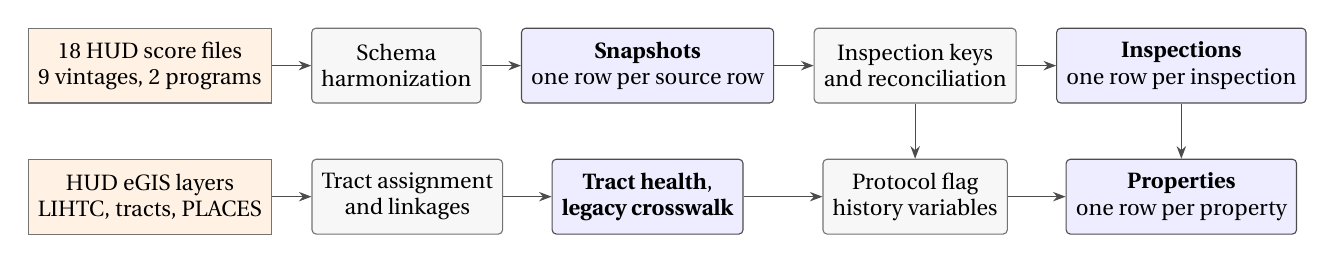
\begin{tikzpicture}[font=\footnotesize, node distance=4mm and 5mm,
  box/.style={draw=black!55, rounded corners=1.5pt, align=center, inner sep=3.5pt, minimum height=9.5mm, fill=black!3},
  outb/.style={draw=black!70, rounded corners=1.5pt, align=center, inner sep=3.5pt, minimum height=9.5mm, fill=blue!7},
  src/.style={draw=black!55, align=center, inner sep=3.5pt, minimum height=9.5mm, fill=orange!10},
  arr/.style={-{Stealth[length=1.6mm]}, black!70}]
\node[src] (raw) {18 HUD score files\\9 vintages, 2 programs};
\node[box, right=of raw] (harm) {Schema\\harmonization};
\node[outb, right=of harm] (snap) {\textbf{Snapshots}\\one row per source row};
\node[box, right=of snap] (key) {Inspection keys\\and reconciliation};
\node[outb, right=of key] (insp) {\textbf{Inspections}\\one row per inspection};
\node[box, below=7mm of key] (prot) {Protocol flag\\history variables};
\node[outb, below=7mm of insp] (prop) {\textbf{Properties}\\one row per property};
\node[src, below=7mm of raw] (gis) {HUD eGIS layers\\LIHTC, tracts, PLACES};
\node[box, right=of gis] (link) {Tract assignment\\and linkages};
\node[outb, below=7mm of snap] (aux) {\textbf{Tract health},\\\textbf{legacy crosswalk}};
\draw[arr] (raw) -- (harm); \draw[arr] (harm) -- (snap); \draw[arr] (snap) -- (key); \draw[arr] (key) -- (insp);
\draw[arr] (insp) -- (prop); \draw[arr] (key) -- (prot); \draw[arr] (prot) -- (prop);
\draw[arr] (gis) -- (link); \draw[arr] (link) -- (aux); \draw[arr] (aux) -- (prot);
\end{tikzpicture}
\caption{AHCP build. Orange boxes are public inputs, grey boxes are processing steps, and blue boxes are released tables. The snapshot table preserves every source row with its file and row number, so each value in the inspection and property tables can be traced to its origin. Linkage attributes are attached to the property table.}\label{fig:pipeline}
\end{figure*}

Figure~\ref{fig:pipeline} summarizes the build. This section states each rule; the released code implements them in six numbered scripts.

\subsection{Formulation}
Let $\mathcal{V}$ be the set of vintages and $g\in\{\mathrm{PH},\mathrm{MF}\}$ the program. Vintage $v$ of program $g$ is a multiset of listings
\begin{equation}
L_{g,v}=\{(p,\,i,\,d,\,s,\,a)\},
\end{equation}
where $p$ is the property identifier, $i$ the HUD inspection identifier (absent in 2011), $d$ the inspection date, $s$ the score, and $a$ a vector of property attributes as stated in that vintage. HUD's own system holds, for each property, a complete sequence of inspections. Each published vintage is a truncated view of it: the last $k_v$ inspections per property as of the release date, with $k_{2011}\le 10$, $k_{2015}\le 3$, and $k_v=1$ thereafter. The reconstruction target is the set of distinct inspections observed in any vintage,
\begin{equation}
\mathcal{I}_g=\Bigl(\bigcup_{v\in\mathcal{V}} L_{g,v}\Bigr)\Big/\sim,
\end{equation}
where $\sim$ identifies listings of the same inspection. $\mathcal{I}_g$ is a subset of the true inspection history, and the complement is not observable from the public files. Sections~\ref{sec:censor} and~\ref{sec:limits} quantify what can be said about it.

\subsection{Schema Harmonization}
Each file is read with all cells as text, to prevent type inference from altering identifiers, and mapped to a single schema using the rules in Table~\ref{tab:schema}. Rows lacking a property identifier, date, or score are dropped, as are exact duplicate rows within a file; in v1.0 neither rule removes any row. The result is the snapshot table: \SSnapshotRows{} rows, one per source row, each carrying \col{source\_file} and \col{source\_row}.

\subsection{Identifiers and the Equivalence Relation}
\subsubsection{Properties} The property key is \col{ahcp\_property\_id} $=g{:}p$. Multifamily properties use the nine-digit identifier of HUD's Real Estate Management System throughout, and it is stable across vintages. Public housing is not: the 2011 file is keyed mostly on pre-2008 project numbers, while later files use eleven-character asset-management development numbers. HUD regrouped projects into developments, often many to one, and the score files contain no crosswalk. AHCP records the scheme of each identifier (\col{id\_scheme}) and does not merge across schemes (Section~\ref{sec:legacy}).

\subsubsection{Inspections} Two listings are identified ($\sim$) when they share program and HUD inspection identifier. For the 2011 file, which has no identifier, listings are identified when they share program, property, and date. Two refinements keep the relation from merging distinct events. First, three property-days in the 2011 file carry two different scores; both are kept, the second with a sequence suffix. Second, one HUD inspection identifier is listed under two developments in the same file with the same score, which we read as a joint inspection; each development keeps its own row and the pair is flagged (\col{shared\_inspection\_id}). The 2011 and 2015 files do not overlap in practice (one 2015 listing per program predates December 2009, and neither matches a 2011 listing), so no identification across the two keying schemes is required.

\subsection{Reconciliation Across Vintages}\label{sec:reconcile}
An inspection listed in several vintages should carry the same score and date in each. When it does not, AHCP keeps the value from the most recent vintage that lists it and retains the minimum and maximum score, the earliest date, and conflict flags. The rule rests on an interpretation, that later files incorporate corrections such as technical reviews and appeals; Section~\ref{sec:reconresults} reports the evidence for it, and the snapshot table lets a user apply a different rule.

\subsection{Protocol Classification}
For an inspection $x$ with date $d_x$ and identifier $i_x$, let $\tau_g$ be the NSPIRE effective date for program $g$ (July~1, 2023 for PH; October~1, 2023 for MF). The protocol is
\begin{equation}
\pi(x)=\begin{cases}
\text{HUD's flag}, & x \text{ listed in the 2025 or 2026 file},\\
\text{NSPIRE}, & \text{else if } i_x \text{ begins \texttt{INSP-}},\\
\text{UPCS}, & \text{else if } d_x<\tau_g,\\
\text{unknown}, & \text{otherwise},
\end{cases}
\end{equation}
and \col{protocol\_source} records which branch applied. In the files that carry HUD's flag, the \col{INSP-} prefix coincides with the NSPIRE flag without exception, which motivates the second branch; in v1.0 that branch and the fourth are never reached.

\subsection{History Variables}
Within each property, inspections are ordered by date and given a sequence number, the previous inspection's date, score and protocol, the interval in days, the score change, and an indicator that the previous inspection used the other protocol. These describe AHCP's records. Because inspections are missing, ``previous'' means previous among those observed.

\subsection{Census Tract Assignment}\label{sec:tract}
Properties are assigned to 2020 census tracts by testing HUD's published coordinates against tract polygons. To keep the build free of compiled geospatial dependencies, the shapefile is parsed directly and each point is tested with the even-odd ray-crossing rule~\cite{shimrat1962} over all rings of a polygon, which handles holes and multi-part tracts. Tract bounding boxes are indexed on a $0.1^\circ$ grid so that each point is tested against only the tracts whose boxes overlap its cell. A point inside no polygon, which occurs along generalized shorelines, is assigned the tract with the nearest boundary vertex if one lies within 1~km, and flagged; otherwise it is left unassigned. Each assignment records its method, and a flag reports whether the tract's county equals the county HUD lists for the property.

\subsection{Subsidy Linkage}
Subsidy attributes are joined exactly on HUD's property or development identifier to the three eGIS layers. A multifamily property present in both the assisted and insured layers takes its attributes from the assisted layer and is marked as present in both. The attributes are a snapshot as of the access date, not a history: they describe the property's current category, program type, unit counts, contract, and financing indicators. Unit counts and occupancy rates of zero in the source are treated as missing.

\subsection{LIHTC Linkage}\label{sec:lihtc}
No shared identifier connects HUD's inspection files to its LIHTC database, so the link is a deterministic record linkage~\cite{fellegi1969,christen2012} in two passes. Addresses on both sides are normalized (case, punctuation, unit designators removed, street-type and directional words abbreviated). Pass one requires equality of normalized street address and five-digit ZIP code. Pass two, for properties unmatched in pass one, accepts a LIHTC project within 50~m whose address begins with the same house number. All matching projects are retained, since tax-credit developments are often financed in phases; the property table reports their number, identifiers, earliest placed-in-service year, and total low-income units, with the pass that produced the match.

\subsection{Legacy Public Housing Crosswalk}\label{sec:legacy}
For each public housing property keyed on a pre-2008 project number, AHCP searches the same agency's later developments for one at the same normalized address and ZIP code or within 50~m. Results are released as a separate candidate table with the method and distance, and the property table carries a candidate only when it is unique. These are leads for a user willing to verify them, not links applied to the panel.

\subsection{Tract Health Estimates}
PLACES crude-prevalence estimates are joined on tract. One geographic change requires handling: PLACES 2025 reports Connecticut tracts under the planning-region county equivalents adopted in 2022, while the 2020 boundary file uses the former counties. The six-digit tract code is unchanged and unique statewide, so Connecticut tracts are re-keyed on it (\placesCT{} properties). The join key is stored separately from the 2020 tract identifier so that neither is altered.

\subsection{Implementation and Reproducibility}
The reference pipeline is written in Python with pandas, NumPy, SciPy, and Matplotlib~\cite{mckinney2010,harris2020,virtanen2020,hunter2007}. Three properties are enforced. (i)~\emph{Provenance}: every raw input is logged with byte length and SHA-256 digest, and every snapshot row carries its source file and row. (ii)~\emph{Determinism}: compressed outputs are written without timestamps, and two consecutive builds from the same inputs produce byte-identical tables. (iii)~\emph{Single source of numbers}: the quality report and a statistics file are written by the pipeline, and the documentation and this article read their figures from those files, so text cannot drift from data. An R package accompanies the release; it reads the released tables and contains a port of the reconstruction step together with a script that compares its output with the Python build. The Python pipeline is the implementation validated here.

\section{Data Records}\label{sec:records}
AHCP v1.0 is deposited at Zenodo~\cite{ahcp} under a CC~BY~4.0 license for data and documentation and an MIT license for code. Table~\ref{tab:records} lists the released tables.

\begin{table}[t]
\caption{Released tables. File names carry the prefix \texttt{ahcp\_}.}\label{tab:records}
\centering\scriptsize\setlength{\tabcolsep}{3.5pt}
\begin{tabular}{@{}llrrr@{}}
\toprule
File & Unit & Rows & Cols. & MB \\
\midrule
\texttt{inspections.csv.gz} & One row per inspection & 313,732 & 25 & 9.2 \\
\texttt{properties.csv} & One row per property & 65,337 & 68 & 28.0 \\
\texttt{snapshots.csv.gz} & One row per source row & 445,664 & 27 & 11.8 \\
\texttt{tract\_health.csv} & One row per tract & 27,890 & 44 & 5.6 \\
\texttt{ph\_legacy\_crosswalk.csv} & Candidate links & 5,439 & 6 & 0.3 \\
\bottomrule
\end{tabular}

\end{table}

\runhead{Inspections.} Keys (\col{ahcp\_inspection\_id}, \col{ahcp\_property\_id}); the HUD identifiers; date, year, score and score scale; protocol and its source; the history variables; the first and last vintage listing the inspection and their count; and the reconciliation fields.

\runhead{Properties.} Identifier and scheme; name, address, county, ZIP code, metropolitan area, coordinates and HUD's location-quality code, each taken from the latest vintage that states it; the vintages in which the property is listed; inspection counts by protocol; and the tract, subsidy, LIHTC, legacy-candidate and health-join fields with their method and quality flags.

\runhead{Snapshots.} The harmonized source rows. This table is the audit trail and the basis for any alternative reconciliation rule.

\runhead{Tract health and legacy crosswalk.} The former holds 40 crude-prevalence measures and two population counts for each tract containing an AHCP property; the latter holds candidate links described in Section~\ref{sec:legacy}.

The panel covers \nStates{} states and territories, \nCounties{} counties and \nTracts{} census tracts; public housing properties belong to \nPHA{} housing agencies. A codebook defines every column with its source and transformation. Appendix~A traces one property through the build.

\section{Technical Validation}\label{sec:validation}
\subsection{Conservation, Uniqueness and Range}
The build asserts, and the quality report records, that (i) the snapshot table has exactly as many rows as were read (\SRawRows{}); (ii) every snapshot row maps to one inspection and every inspection to one property; (iii) inspection and property keys are unique; (iv) no inspection appears twice within a vintage; (v) scores lie in $[0,100]$ and dates between January 2000 and the latest file's stated as-of date; (vi) coordinates fall within U.S. bounds including territories; and (vii) no protocol is left undetermined. A build that violates any of these exits with an error. Four snapshot rows, all in the 2018 vintage, carry inspection dates in the first days of April 2018, after the March 2018 date in that file's title (the file was revised in May 2018); they are retained.

\subsection{Independent Recount and Round Trip}
Two checks do not share code with the pipeline's grouping logic. A recount of distinct (program, inspection identifier, property) triples plus distinct identifier-free (program, property, date, score) tuples, computed directly from the raw files, returns \SInspections{}, the number of rows in the inspection table. Separately, the two 2026 workbooks are re-read with a spreadsheet library alone; every one of their \curProps{} inspections is present in AHCP with an identical score.

\subsection{Cross-Vintage Reconciliation}\label{sec:reconresults}
Of \SInspections{} inspections, \inspMultiVintage{} are listed in more than one vintage (up to \inspMaxVintages{}). Among these, \SScoreConflicts{} (\scoreConfPctMulti\%) carry different scores in different vintages and \SDateConflicts{} (\dateConfPctMulti\%) different dates. The date differences are mostly trivial: \dateConfOneDay{} are exactly one day, concentrated between the 2015 file, which reports times of day, and later files. The score differences are informative. In \scoreConfUp{} of the \SScoreConflicts{} cases the later vintage reports the higher score and in \scoreConfDown{} the lower (Fig.~\ref{fig:revisions}); the median absolute revision is \scoreConfMedian{} points, and \scoreConfCrossSixty{} revisions move an inspection across the passing score of 60. A pattern of rare, almost uniformly upward revisions is what the appeal and technical-review processes would produce, and it supports the choice to keep the latest value. It is not confirmation: HUD's files do not state why a score changed.

\begin{figure}[t]
\centering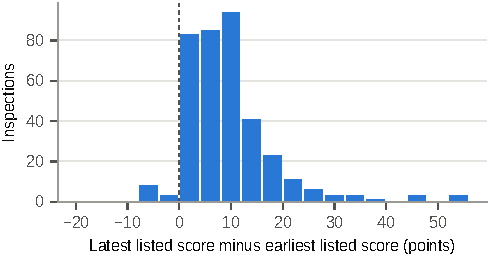
\includegraphics[width=\columnwidth]{figs/revisions.pdf}
\caption{Score revisions between vintages for the \SScoreConflicts{} inspections whose listed score changed. Positive values mean the later file reports a higher score. Values beyond the axis limits are placed in the end bins.}\label{fig:revisions}
\end{figure}

\subsection{Coverage and Censoring}\label{sec:censor}
\begin{figure}[t]
\centering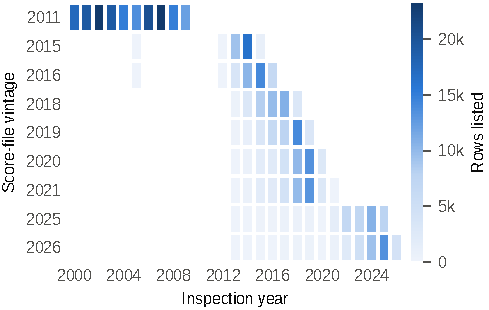
\includegraphics[width=\columnwidth]{figs/window.pdf}
\caption{Rows listed in each score-file vintage by inspection year, both programs. Blank cells contain no rows. The 2011 file is a history file; each later file is a narrow window ending at its release date.}\label{fig:window}
\end{figure}
\begin{figure}[t]
\centering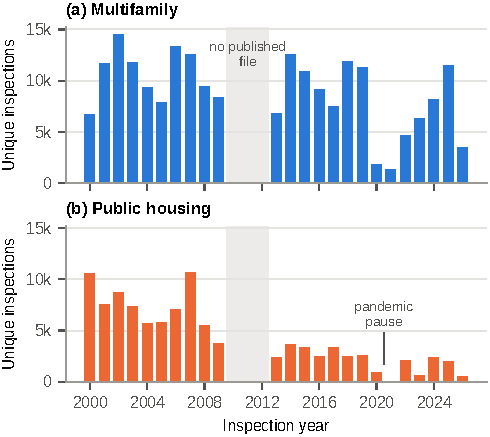
\includegraphics[width=\columnwidth]{figs/coverage.pdf}
\caption{Unique inspections in AHCP by inspection year. The shaded band marks 2010 to 2012, which no published file covers.}\label{fig:coverage}
\end{figure}

Fig.~\ref{fig:window} shows each vintage as a window onto inspection years, and Fig.~\ref{fig:coverage} the resulting coverage. Three features define what the panel can support.

\runhead{The 2010--2012 gap.} The 2011 file ends in November 2009 and the 2015 file effectively begins in 2013. AHCP holds \SInspectionsTwentytenTwentytwelve{} inspections dated 2010 to 2012. These years are absent from the public record, not sparsely covered.

\runhead{Single-vintage survival.} Table~\ref{tab:firstvintage} attributes each inspection to the first vintage that lists it. The 2011 file contributes \inspLegacy{} inspections. Of the \inspPostLegacy{} that first appear later, \inspPostOneVintage{} (\pctPostOneVintage\%) are listed in exactly one vintage: had that one file not been posted, or not been retained, they would be unrecoverable. This is the direct measure of how fragile the public record is.

\begin{table}[t]
\caption{Unique inspections by the first vintage that lists them}\label{tab:firstvintage}
\centering\footnotesize
\begin{tabular}{lrrrr}
\toprule
First vintage & PH & MF & Total & \% \\
\midrule
2011 & 72,515 & 105,471 & 177,986 & 56.7 \\
2015 & 6,464 & 19,869 & 26,333 & 8.4 \\
2016 & 4,822 & 14,781 & 19,603 & 6.2 \\
2018 & 4,332 & 14,466 & 18,798 & 6.0 \\
2019 & 2,648 & 11,795 & 14,443 & 4.6 \\
2020 & 2,724 & 10,852 & 13,576 & 4.3 \\
2021 & 1 & 14 & 15 & 0.0 \\
2025 & 5,640 & 27,499 & 33,139 & 10.6 \\
2026 & 1,891 & 7,948 & 9,839 & 3.1 \\
\midrule
Total & 101,037 & 212,695 & 313,732 & 100.0 \\
\bottomrule
\end{tabular}

\end{table}

\runhead{Turnover between vintages.} Table~\ref{tab:persistence} reports, for consecutive vintages, the share of properties retained and, among those retained, the share whose listed inspection changed. Between the 2020 and 2021 files no retained property shows a new inspection, consistent with the suspension of inspections during the pandemic. Between the 2021 and 2025 files more than nine in ten retained properties show a different inspection. Whatever inspections occurred in between and were themselves superseded before August 2025 are lost.

\begin{table}[t]
\caption{Turnover between consecutive vintages. Retained: share of the earlier vintage's properties listed in the later one. New insp.: among retained properties, share whose listed inspection differs.}\label{tab:persistence}
\centering\footnotesize
\resizebox{\columnwidth}{!}{\begin{tabular}{lrrrrrr}
\toprule
Vintage pair & PH props. & Retained (\%) & New insp. (\%) & MF props. & Retained (\%) & New insp. (\%) \\
\midrule
2015 $\rightarrow$ 2016 & 5,800 & 95.4 & 56.0 & 18,737 & 96.9 & 34.5 \\
2016 $\rightarrow$ 2018 & 7,257 & 93.7 & 61.9 & 26,672 & 97.7 & 49.0 \\
2018 $\rightarrow$ 2019 & 6,923 & 97.2 & 38.5 & 27,755 & 98.6 & 41.2 \\
2019 $\rightarrow$ 2020 & 6,783 & 97.2 & 40.7 & 27,878 & 97.7 & 37.3 \\
2020 $\rightarrow$ 2021 & 6,638 & 98.3 & 0.0 & 27,925 & 98.2 & 0.0 \\
2021 $\rightarrow$ 2025 & 6,524 & 92.2 & 90.9 & 27,419 & 94.0 & 96.3 \\
2025 $\rightarrow$ 2026 & 6,190 & 98.9 & 30.7 & 28,459 & 99.4 & 26.3 \\
\bottomrule
\end{tabular}
}
\end{table}

\runhead{Observed intervals.} Table~\ref{tab:intervals} summarizes the time between consecutive inspections of the same property as observed in AHCP. Within the history file the median interval is \ivMedPHA{} years for public housing and \ivMedMFA{} for multifamily, in line with a schedule of one to three years. Within 2013 to 2019 the medians are \ivMedPHB{} and \ivMedMFB{} years, and \ivLongMFB\% of multifamily intervals exceed 3.5 years, longer than the schedule alone would produce. For intervals ending in 2020 or later the medians rise to \ivMedPHC{} and \ivMedMFC{} years and most exceed 3.5 years. These long intervals combine a real pause in inspections with inspections that occurred but were never captured in a published file; the public data cannot separate the two.

\begin{table}[t]
\caption{Years between consecutive inspections of the same property as observed in AHCP}\label{tab:intervals}
\centering\footnotesize
\resizebox{\columnwidth}{!}{\begin{tabular}{llrrrrr}
\toprule
Interval & Prog. & Pairs & P25 & Median & P75 & $>$3.5 y (\%) \\
\midrule
Within 2000--2009 & PH & 52,423 & 1.13 & 1.71 & 2.18 & 2.5 \\
 & MF & 73,262 & 1.08 & 2.01 & 2.99 & 10.9 \\
Across the 2010--2012 gap & PH & 4,816 & 4.57 & 5.14 & 5.91 & 99.9 \\
 & MF & 23,406 & 5.53 & 6.45 & 7.53 & 99.9 \\
Within 2013--2019 & PH & 12,388 & 1.47 & 2.05 & 2.86 & 4.2 \\
 & MF & 39,949 & 1.57 & 2.34 & 3.15 & 12.9 \\
Ending 2020--2026 & PH & 8,200 & 2.90 & 4.14 & 5.51 & 60.9 \\
 & MF & 33,951 & 3.31 & 4.61 & 6.06 & 70.4 \\
\bottomrule
\end{tabular}
}
\end{table}

The practical consequence is that AHCP supports statements about observed inspections and lower bounds on change, and does not support statements that a property was \emph{not} inspected or did \emph{not} fail in a period.

\subsection{Protocol Flags}
HUD's flag covers \SNspireHudFlag{} NSPIRE and \SUpcsHudFlag{} UPCS inspections; \SUpcsInferred{} are labelled UPCS by date. No flagged UPCS inspection postdates its program's NSPIRE effective date. HUD flags \SNspireMfBeforeStart{} multifamily inspections as NSPIRE that are dated before October~1, 2023, the earliest in June 2023; these keep HUD's flag. The inferred labels apply almost entirely to inspections from 2000 to 2021, years before NSPIRE scoring existed, so the inference carries little risk; the exception would be an NSPIRE inspection conducted after the effective date, superseded, and never listed in a flagged file, and such an inspection is by construction absent from the panel.

\subsection{Geocoding}
Of \SProperties{} properties, \tractContains{} fall inside a tract polygon, \tractNearest{} are assigned by the nearest-vertex fallback, \tractOutside{} lie beyond 1~km of any tract, and \tractNoCoord{} have no coordinates; nearly all of the last group appear only in the 2011 file. Among properties in the 2026 vintage, \curTractPct\% receive a tract. Two references that play no part in the assignment check the result. The county implied by the assigned tract equals the county HUD lists in \tractCountyAgree{} of \tractCountyN{} comparable cases (\STractCountyAgreePct\%). And for \tractHudCompareN{} properties where HUD's eGIS layers supply a 2010 tract code, the 2020 tract assigned here has the same eleven-digit code in \tractHudSameCode\% of cases and the same county in \tractHudSameCounty\%; disagreement in code largely reflects tracts that were split or renumbered between censuses, so the figure is a lower bound on agreement. HUD's location-quality code shows that \lqRooftopPct\% of current properties are geocoded to an interpolated rooftop position, \lqZipFourPct\% to a ZIP+4 centroid, \lqBlockGroupPct\% to a block-group centroid, and \lqZipCentroidPct\% to a ZIP Code centroid; HUD's dictionary warns that county and metropolitan codes are unreliable for the last group, and the same caution applies to tracts.

\subsection{Linkage Coverage and Accuracy}
\begin{table}[t]
\caption{Linkage coverage}\label{tab:linkage}
\centering\footnotesize
\resizebox{\columnwidth}{!}{\begin{tabular}{lrrrr}
\toprule
Linkage & All properties & \% & In 2026 vintage & \% \\
\midrule
Census tract (2020) & 59,716 & 91.4 & 34,920 & 100.0 \\
HUD subsidy record & 34,997 & 53.6 & 34,628 & 99.2 \\
LIHTC project & 6,110 & 9.4 & 4,739 & 13.6 \\
PLACES tract estimates & 58,803 & 90.0 & 34,376 & 98.4 \\
\bottomrule
\end{tabular}
}
\end{table}
Table~\ref{tab:linkage} reports coverage. The subsidy join is exact and nearly complete for current properties; its low coverage over all properties reflects that properties no longer in HUD's current layers, including all pre-2008 public housing projects, cannot be matched. PLACES coverage is limited by its geography: unmatched tract-coded properties are almost all in Puerto Rico and other territories.

The LIHTC link can be assessed against an imperfect reference. HUD's multifamily layers carry a tax-credit indicator on the primary assistance contract, populated for a subset of properties. Among properties where that indicator is affirmative, AHCP links \lihtcSens\% (\lihtcYLinked{} of those flagged); where it is negative, AHCP links \lihtcFalse\% (\lihtcNLinked{}). Read as a classifier against HUD's indicator, the link has modest sensitivity and a low false-link rate; among linked properties with a populated indicator, \lihtcPPV\% have an affirmative one. The indicator is itself incomplete and the LIHTC layer was last updated in December 2024, so neither figure is an error rate in the strict sense. The link is suitable for identifying properties that certainly have tax-credit financing at a matched address and unsuitable for estimating the share that do.

The legacy crosswalk finds at least one candidate for \legacyAny{} of \legacyTotal{} pre-2008 projects (\legacyAnyPct\%) and exactly one for \legacyUnique{}. Its accuracy has not been assessed against an external reference.

\section{Descriptive Results}\label{sec:results}
The statistics in this section describe the inspections AHCP observes. They are offered to characterize the dataset, and none is an estimate of a causal effect.

\subsection{Score Distributions}
\begin{table*}[t]
\caption{Inspection scores by program, period and protocol. P10 and P90 are the 10th and 90th percentiles; the last two columns are the shares of inspections scoring below 60 and at or above 90.}\label{tab:desc}
\centering\footnotesize
\begin{tabular}{lllrrrrrrrr}
\toprule
Prog. & Period & Protocol & $n$ & Mean & SD & P10 & Median & P90 & $<$60 (\%) & $\geq$90 (\%) \\
\midrule
PH & 2000--2009 & UPCS & 72,516 & 80.4 & 15.5 & 58.6 & 84.1 & 97.0 & 11.1 & 33.2 \\
PH & 2012--2023 & UPCS & 23,579 & 81.3 & 15.0 & 60.0 & 85.0 & 97.0 & 9.5 & 37.2 \\
PH & 2023--2026 & NSPIRE & 4,942 & 81.1 & 17.5 & 59.0 & 86.0 & 97.0 & 15.6 & 40.5 \\
MF & 2000--2009 & UPCS & 105,471 & 81.5 & 15.0 & 60.9 & 85.0 & 97.5 & 9.2 & 35.7 \\
MF & 2012--2023 & UPCS & 83,232 & 85.1 & 12.8 & 67.0 & 89.0 & 98.0 & 4.6 & 46.7 \\
MF & 2023--2026 & NSPIRE & 23,992 & 88.9 & 12.4 & 75.0 & 93.0 & 99.0 & 4.4 & 63.3 \\
\bottomrule
\end{tabular}

\end{table*}
\begin{figure*}[t]
\centering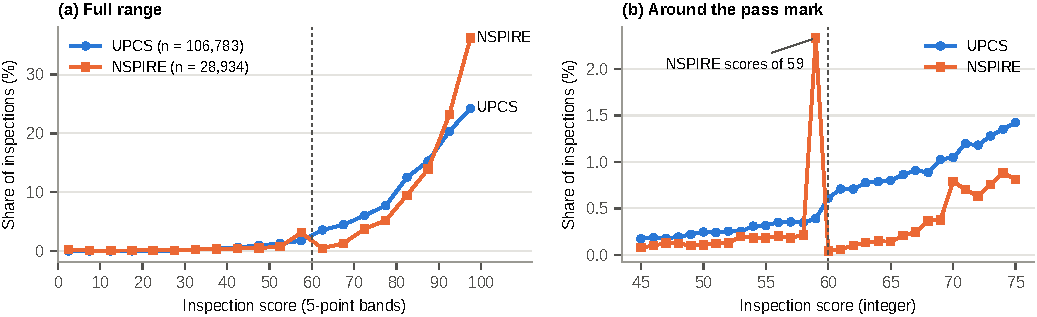
\includegraphics[width=\textwidth]{figs/scores.pdf}
\caption{Score distributions by protocol for inspections dated 2013 onward. (a) Shares in five-point bands. (b) Shares at each integer score from 45 to 75. The vertical dashed line marks the passing score of 60. Scores are as published; AHCP does not rescale across protocols.}\label{fig:scores}
\end{figure*}

Table~\ref{tab:desc} and Fig.~\ref{fig:scores} summarize scores. Three observations follow. First, public housing scores are lower and more dispersed than multifamily scores in every period, and the share of failing inspections is higher: \failPHUPCSB\% against \failMFUPCSB\% under UPCS in 2012 to 2023, and \failPHNSPIREB\% against \failMFNSPIREB\% under NSPIRE. Second, multifamily scores under NSPIRE are concentrated at the top: \meanMFNSPIREB{} on average against \meanMFUPCSB{} for multifamily UPCS inspections in 2012 to 2023. Third, the lower tail has a different shape under NSPIRE. Under UPCS the density rises smoothly through the passing score. Under NSPIRE, \nspirePctFiftyNine\% of all scores (\nspireAtFiftyNine{} inspections) are exactly 59, the band from 60 to 64 is nearly empty (\nspireSixtyToSixtyFour\% against \upcsSixtyToSixtyFour\% under UPCS), and the public housing failure share is \failPHNSPIREB\% against \failPHUPCSB\%. The spike at 59 is the unit-threshold rule of the scoring notice~\cite{nspirescoring}: a property that would otherwise pass is assigned 59 when unit deficiencies exceed the threshold. A score of 59 under NSPIRE therefore does not mean ``one point short''. Any analysis that treats the score as a continuous measure near the threshold, such as a regression discontinuity at 60, must account for this.

\subsection{Consecutive Inspections and the Protocol Change}
\SPropertiesBothProtocols{} properties have at least one inspection under each protocol. Table~\ref{tab:transitions} compares consecutive observed inspections of the same property by the protocols of the pair, and Fig.~\ref{fig:change} shows the distribution of score changes.

\begin{table*}[t]
\caption{Consecutive observed inspections of the same property, by protocol of the earlier and later inspection (earlier inspection dated 2013 or later). $r$ is the Pearson correlation between the two scores. Pass$\to$fail is the share of all pairs moving from 60 or above to below 60; fail$\to$pass is the share of pairs starting below 60 that end at 60 or above.}\label{tab:transitions}
\centering\footnotesize
\begin{tabular}{llrrrrrrrr}
\toprule
Pair type & Prog. & Pairs & Prev. mean & Next mean & Mean $\Delta$ & SD $\Delta$ & $r$ & Pass$\to$fail (\%) & Fail$\to$pass (\%) \\
\midrule
UPCS $\rightarrow$ UPCS & PH & 15,717 & 81.0 & 79.1 & $-$1.8 & 15.3 & 0.49 & 7.8 & 56.5 \\
 & MF & 52,094 & 83.9 & 84.4 & 0.5 & 14.6 & 0.37 & 3.7 & 80.2 \\
UPCS $\rightarrow$ NSPIRE & PH & 4,457 & 80.3 & 81.8 & 1.6 & 19.3 & 0.32 & 11.0 & 69.2 \\
 & MF & 20,746 & 87.2 & 89.3 & 2.1 & 14.4 & 0.22 & 3.7 & 88.1 \\
NSPIRE $\rightarrow$ NSPIRE & PH & 388 & 60.8 & 71.7 & 10.9 & 21.8 & 0.27 & 8.2 & 62.1 \\
NSPIRE $\rightarrow$ NSPIRE & MF & 1,060 & 71.0 & 83.0 & 12.0 & 19.0 & 0.18 & 6.7 & 87.0 \\
\bottomrule
\end{tabular}

\end{table*}
\begin{figure}[t]
\centering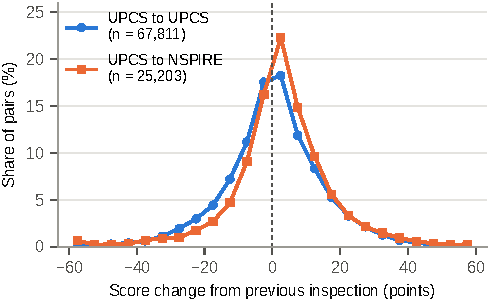
\includegraphics[width=\columnwidth]{figs/change.pdf}
\caption{Change in score between consecutive observed inspections of the same property, in five-point bands, for pairs within UPCS and pairs spanning the change to NSPIRE.}\label{fig:change}
\end{figure}

Scores are only moderately persistent. Within UPCS the correlation between consecutive scores is \trUUPHR{} for public housing and \trUUMFR{} for multifamily; across the protocol change it is \trUNPHR{} and \trUNMFR{}. The lower cross-protocol correlation has at least two sources that the table cannot separate: the scoring model changed, and the pairs spanning the change are further apart in time (median \trUNgapMedian{} years against \trUUgapMedian{} within UPCS). Mean changes are small in both cases. Among public housing pairs spanning the change, \trUNPHNewFail\% move from passing to failing, against \trUUPHNewFail\% within UPCS.

The NSPIRE-to-NSPIRE rows illustrate selection. Their earlier scores average far below the population and are followed by mean gains of \trNNPHDelta{} (public housing) and \trNNMFDelta{} (multifamily) points, because within three years of a new protocol the properties with two NSPIRE inspections are disproportionately those reinspected early after a low score, and because a low observed score is followed by a higher one through regression to the mean~\cite{barnett2005} as well as through repair. The same caution applies to every fail-to-pass figure in the table.

\subsection{Current Portfolio by Subsidy Category}
\begin{table}[t]
\caption{Properties listed in the 2026 vintage by HUD subsidy category, with their latest observed score. Categories with fewer than 100 properties are omitted.}\label{tab:subsidy}
\centering\footnotesize
\resizebox{\columnwidth}{!}{\begin{tabular}{lrrrrrr}
\toprule
Subsidy category & Properties & Median units & Mean score & Median & $<$60 (\%) & NSPIRE (\%) \\
\midrule
202/811 & 6,235 & 18.0 & 91.8 & 95.0 & 2.1 & 84.6 \\
Public Housing & 6,117 & 100.0 & 84.0 & 89.0 & 9.6 & 74.0 \\
Insured-Unsubsidized & 5,837 & 111.0 & 88.8 & 92.0 & 3.6 & 77.4 \\
Subsidized - Previously Insured & 5,229 & 86.0 & 88.1 & 92.0 & 4.5 & 79.0 \\
Insured-Subsidized & 4,854 & 85.0 & 91.2 & 94.0 & 1.8 & 77.1 \\
Subsidized, No HUD Financing & 4,466 & 44.0 & 89.0 & 92.0 & 3.8 & 80.4 \\
Subsidized - Previously 202/811 & 1,598 & 23.5 & 92.2 & 95.0 & 1.5 & 80.9 \\
Not in current HUD layers & 294 & -- & 82.0 & 89.0 & 12.6 & 29.6 \\
HUD Held & 201 & 55.0 & 85.7 & 91.0 & 9.0 & 78.1 \\
\bottomrule
\end{tabular}
}
\end{table}
The 2026 vintage lists \curProps{} properties (\curMF{} multifamily, \curPH{} public housing); \curNspirePct\% have a latest inspection under NSPIRE and \curFailN{} (\curFailPct\%) a latest score below 60. Table~\ref{tab:subsidy} breaks these down by HUD's subsidy category. Supportive housing for the elderly and persons with disabilities (Section~202/811, current and former) and insured-subsidized properties show the highest scores and the lowest failure shares; public housing and HUD-held properties show the lowest scores. The table mixes protocols and inspection years, and the multifamily file includes insured properties without rental subsidy, so the rows are not a ranking of programs.

\subsection{Neighborhood Context: An Illustration of the Health Linkage}
To illustrate the tract linkage, Table~\ref{tab:context} groups current properties whose latest inspection is under NSPIRE by quartile of their tract's PLACES estimate of housing insecurity. Properties in tracts with the highest estimated housing insecurity have a latest failure share of \ctxFailHigh\%, against \ctxFailLow\% in the lowest quartile, and the rank correlation between the tract estimate and the property's score is \ctxSpearman{}.

\begin{table}[t]
\caption{Current properties with a latest NSPIRE inspection, by quartile of tract housing insecurity (CDC PLACES 2025, crude prevalence among adults). Asthma is the mean tract prevalence of current asthma.}\label{tab:context}
\centering\footnotesize
\resizebox{\columnwidth}{!}{\begin{tabular}{lrrrrr}
\toprule
Tract housing-insecurity quartile & Properties & Range (\%) & Asthma (\%) & Mean score & $<$60 (\%) \\
\midrule
Q1 (lowest) & 5,149 & 2.9--10.3 & 10.3 & 91.1 & 2.4 \\
Q2 & 5,136 & 10.4--14.9 & 10.9 & 90.2 & 3.4 \\
Q3 & 5,182 & 15.0--23.5 & 11.4 & 88.6 & 5.0 \\
Q4 (highest) & 5,098 & 23.6--56.8 & 12.6 & 85.3 & 8.9 \\
\bottomrule
\end{tabular}
}
\end{table}

This is an ecological description and nothing more~\cite{robinson1950}. PLACES estimates are model based, describe all adults in a tract, and are not estimates for residents of assisted housing; the association may reflect where older or under-capitalized properties are located, how inspection outcomes vary with building type, or both. The table shows that the linkage is usable and that building condition and neighborhood disadvantage are not independent in these data.

\section{Usage Notes}\label{sec:usage}
\runhead{Start from the inspection table and join properties on the key.} Read identifier, ZIP and FIPS columns as text to preserve leading zeros.

\runhead{Treat the panel as left- and interval-censored.} Counts of inspections per property, intervals, and ``first failure'' dates are functions of which vintages happened to be published. Analyses of timing should condition on a property being observable, for example by restricting to properties listed in a given pair of vintages, and should not interpret long observed intervals as long true intervals.

\runhead{Do not pool levels across protocols.} Include protocol as a stratifier or model term. For comparisons across 2023, consider within-protocol ranks or pass/fail status, and handle the mass at 59 explicitly. The \SPropertiesBothProtocols{} properties observed under both protocols are the natural basis for a bridging study, which AHCP does not attempt.

\runhead{Use the flags.} \col{score\_conflict}, \col{date\_conflict\_days}, \col{protocol\_source}, \col{tract\_method}, \col{tract\_county\_agrees}, \col{location\_quality} and \col{lihtc\_match\_type} exist so that a sensitivity analysis is one filter away.

\runhead{Treat subsidy attributes as current.} They describe the property at the access date. Attaching them to inspections from earlier years assumes the category did not change.

\runhead{Keep public housing eras separate unless the crosswalk has been verified.} Analyses spanning 2009 and 2013 for public housing should either restrict to developments keyed consistently or verify candidates in the crosswalk table.

\runhead{Rebuild or extend.} New vintages are added by registering their URLs in the source manifest and re-running the numbered scripts; the quality report will show any change in the inputs.

\section{Limitations}\label{sec:limits}
\begin{enumerate}
\item \textbf{Incomplete histories.} AHCP contains the inspections that survive in a published file. No file covers 2010 to 2012, and from 2016 on a superseded inspection is lost unless a vintage happened to capture it. The size of the unobserved set is unknown.
\item \textbf{History variables are conditional on observation.} Sequence numbers, intervals, and score changes skip unobserved inspections.
\item \textbf{No cross-protocol comparability.} UPCS and NSPIRE scores come from different models; AHCP reports both as published.
\item \textbf{Reconciliation rests on an interpretation.} Keeping the latest listed score is supported by the direction of revisions but not confirmed by HUD documentation.
\item \textbf{Identifier discontinuity in public housing.} \SPropertiesPhPreAmp{} properties appear only under pre-2008 project numbers. The crosswalk is unvalidated.
\item \textbf{One point per property.} Scattered-site developments and multi-building properties are represented by a single address, coordinate pair, and tract. Tract assignment inherits HUD's geocoding quality and uses generalized boundaries.
\item \textbf{Linkage limits.} Subsidy attributes are a current snapshot. The LIHTC link is conservative and incomplete; a non-link is not evidence of no tax credit. PLACES estimates are modeled, tract-wide, from a single release, and absent for the territories.
\item \textbf{The score is the protocol's measure.} It is not a complete measure of housing quality or of residents' experience, and prior reviews have identified weaknesses in the inspection process itself~\cite{gao2019,oig2024}.
\item \textbf{Mutable sources.} HUD replaces files in place. The provenance log fixes the inputs of this release; a rebuild from later downloads may differ.
\item \textbf{Software scope.} The Python pipeline is the validated implementation. The R port of the reconstruction step is released with a comparison script and should be checked with it before use.
\end{enumerate}

\section{Conclusion}
The public record of HUD physical inspections is overwritten by design, but enough of it remains to rebuild a substantial panel: \SInspections{} inspections of \SProperties{} properties over 26 years, spanning the change of inspection protocol. AHCP v1.0 releases that panel with the rules that produced it, the evidence for those rules, and a measured account of what is missing. The reconstruction also yields three findings about the record itself: over a third of post-2012 inspections survive in a single file, score revisions between files are rare and almost always upward, and NSPIRE scores carry a rule-induced mass at 59 that changes how the passing threshold should be analyzed. The release is designed to be extended as HUD posts new vintages. Recovering the missing years would require archived copies of intermediate files or records from HUD directly, and a validated bridge between UPCS and NSPIRE scores remains future work.

\section*{Data and Code Availability}
AHCP v1.0 is archived at Zenodo, \url{https://doi.org/10.5281/zenodo.23200319} (all versions: \url{https://doi.org/10.5281/zenodo.23200318}), with source at \url{https://github.com/AYISHATUAMEEN/ahcp}. The archive contains the five tables, the codebook, the limitations document, the quality report, the provenance log, the pipeline, the scripts that generate every number, table and figure in this article, and the R package. All inputs are public U.S. Government works available from the cited sources.

\section*{Acknowledgment}
The author thanks the agencies that publish the underlying data. AHCP is not endorsed by HUD, the Census Bureau, or CDC. \emph{Use of AI tools:} code, data processing, figures, and a draft of this manuscript were prepared with the assistance of Claude (Anthropic). The author directed the work, reviewed the code and outputs, verified results against the source files, and is responsible for all content. The author declares no competing interests.


\begin{thebibliography}{99}\footnotesize\setlength{\itemsep}{0pt}\setlength{\parskip}{0pt}
\bibitem{krieger2002} J. Krieger and D. L. Higgins, ``Housing and health: time again for public health action,'' \emph{Amer. J. Public Health}, vol. 92, no. 5, pp. 758--768, 2002.
\bibitem{jacobs2011} D. E. Jacobs, ``Environmental health disparities in housing,'' \emph{Amer. J. Public Health}, vol. 101, no. S1, pp. S115--S122, 2011.
\bibitem{swope2019} C. B. Swope and D. Hern\'andez, ``Housing as a determinant of health equity: a conceptual model,'' \emph{Soc. Sci. Med.}, vol. 243, Art. no. 112571, 2019.
\bibitem{cfr5g} U.S. Department of Housing and Urban Development, ``Physical condition standards and inspection requirements,'' 24 C.F.R. pt. 5, subpt. G.
\bibitem{gao2019} U.S. Government Accountability Office, ``Real Estate Assessment Center: HUD should improve physical inspection process and oversight of inspectors,'' GAO-19-254, Mar. 2019.
\bibitem{hudpis} U.S. Department of Housing and Urban Development, Office of Policy Development and Research, ``Physical inspection scores,'' dataset. [Online]. Available: \url{https://www.huduser.gov/portal/datasets/pis.html} (accessed Oct. 6, 2026).
\bibitem{gao2001} U.S. General Accounting Office, ``HUD inspections: steps needed to address uncertainty in inspection scores,'' GAO-01-109, 2000.
\bibitem{oig2024} U.S. Department of Housing and Urban Development, Office of Inspector General, ``HUD lacked adequate oversight of multifamily housing properties with failing REAC scores or life-threatening deficiencies,'' Audit Rep. 2024-CH-0001, Feb. 2024.
\bibitem{nspirerule} U.S. Department of Housing and Urban Development, ``Economic Growth Regulatory Relief and Consumer Protection Act: implementation of National Standards for the Physical Inspection of Real Estate (NSPIRE),'' final rule, 88 Fed. Reg. 30442, May 11, 2023.
\bibitem{nspirescoring} U.S. Department of Housing and Urban Development, ``National Standards for the Physical Inspection of Real Estate and associated protocols, scoring notice,'' 88 Fed. Reg. 43371, July 7, 2023.
\bibitem{ahcp} A. Ameen, ``Assisted Housing Condition Panel (AHCP) v1.0: harmonized HUD public housing and multifamily physical inspection scores, 2000--2026,'' Zenodo, dataset, 2026, doi: 10.5281/zenodo.23200319.
\bibitem{fr2000} U.S. Department of Housing and Urban Development, notice on the physical inspection scoring process, 65 Fed. Reg. 77230, 2000 (cited in HUD's multifamily data dictionary).
\bibitem{fr2001} U.S. Department of Housing and Urban Development, notice on the Public Housing Assessment System physical condition scoring process, 66 Fed. Reg. 59084, 2001 (cited in HUD's public housing data dictionary).
\bibitem{cfr200857} U.S. Department of Housing and Urban Development, ``Administrative process for scoring and ranking the physical condition of multifamily housing properties,'' 24 C.F.R. \S~200.857.
\bibitem{datalumos} ``Office of Policy Development and Research (PD\&R) physical inspection scores,'' DataLumos, Inter-university Consortium for Political and Social Research, 2025, doi: 10.3886/E219244V1.
\bibitem{nhpd} Public and Affordable Housing Research Corporation and National Low Income Housing Coalition, ``National Housing Preservation Database.'' [Online]. Available: \url{https://preservationdatabase.org} (accessed Oct. 6, 2026).
\bibitem{propublica} ProPublica, ``HUD Inspect.'' [Online]. Available: \url{https://projects.propublica.org/hud/} (accessed Oct. 6, 2026).
\bibitem{hudegis} U.S. Department of Housing and Urban Development, ``HUD eGIS open data.'' [Online]. Available: \url{https://hudgis-hud.opendata.arcgis.com/} (accessed Oct. 6, 2026).
\bibitem{greenlund2022} K. J. Greenlund \emph{et al.}, ``PLACES: local data for better health,'' \emph{Prev. Chronic Dis.}, vol. 19, Art. no. 210459, 2022.
\bibitem{hudlihtc} U.S. Department of Housing and Urban Development, ``Low-Income Housing Tax Credit (LIHTC): property level data.'' [Online]. Available: \url{https://www.huduser.gov/portal/datasets/lihtc.html} (accessed Oct. 6, 2026).
\bibitem{censuscb} U.S. Census Bureau, ``Cartographic boundary files: census tracts, 2020, 1:500,000.'' [Online]. Available: \url{https://www2.census.gov/geo/tiger/GENZ2020/shp/} (accessed Oct. 6, 2026).
\bibitem{places2025} Centers for Disease Control and Prevention, ``PLACES: census tract data (GIS friendly format), 2025 release.'' [Online]. Available: \url{https://data.cdc.gov/d/yjkw-uj5s} (accessed Oct. 6, 2026).
\bibitem{shimrat1962} M. Shimrat, ``Algorithm 112: position of point relative to polygon,'' \emph{Commun. ACM}, vol. 5, no. 8, p. 434, 1962.
\bibitem{fellegi1969} I. P. Fellegi and A. B. Sunter, ``A theory for record linkage,'' \emph{J. Amer. Statist. Assoc.}, vol. 64, no. 328, pp. 1183--1210, 1969.
\bibitem{christen2012} P. Christen, \emph{Data Matching: Concepts and Techniques for Record Linkage, Entity Resolution, and Duplicate Detection}. Berlin, Germany: Springer, 2012.
\bibitem{mckinney2010} W. McKinney, ``Data structures for statistical computing in Python,'' in \emph{Proc. 9th Python in Science Conf.}, 2010, pp. 56--61.
\bibitem{harris2020} C. R. Harris \emph{et al.}, ``Array programming with NumPy,'' \emph{Nature}, vol. 585, pp. 357--362, 2020.
\bibitem{virtanen2020} P. Virtanen \emph{et al.}, ``SciPy 1.0: fundamental algorithms for scientific computing in Python,'' \emph{Nature Methods}, vol. 17, pp. 261--272, 2020.
\bibitem{hunter2007} J. D. Hunter, ``Matplotlib: a 2D graphics environment,'' \emph{Comput. Sci. Eng.}, vol. 9, no. 3, pp. 90--95, 2007.
\bibitem{barnett2005} A. G. Barnett, J. C. van der Pols, and A. J. Dobson, ``Regression to the mean: what it is and how to deal with it,'' \emph{Int. J. Epidemiol.}, vol. 34, no. 1, pp. 215--220, 2005.
\bibitem{robinson1950} W. S. Robinson, ``Ecological correlations and the behavior of individuals,'' \emph{Amer. Sociol. Rev.}, vol. 15, no. 3, pp. 351--357, 1950.
\end{thebibliography}

\clearpage
\onecolumn
\begin{center}\textsc{Appendix: Worked Example, Quality Checks, and Algorithms}\end{center}

\appsection{A}{Worked Example: One Property Through the Build}
Table~\ref{tab:exsnap} shows every listing of one multifamily property (\col{MF:800006156}) in the snapshot table, and Table~\ref{tab:exinsp} the inspections reconstructed from them. The \exSnapRows{} listings reduce to \exInspRows{} inspections. The inspection with HUD identifier 502015 is listed in the 2015 vintage with a score of 72 and a date of March~17, 2014, and in the 2016 vintage with a score of 80 and a date one day later; AHCP keeps the 2016 values, sets \col{score\_conflict} to 1, and retains 72 and 80 as the minimum and maximum. No inspection is observed between February 2008 and March 2014, or between December 2018 and March 2025: the first interval spans the 2010 to 2012 gap and the second the interval between the 2021 and 2025 vintages.

\begin{table}[h]
\caption{Snapshot listings for property MF:800006156}\label{tab:exsnap}
\centering\footnotesize
\begin{tabular}{rrllrl}
\toprule
Vintage & Row & HUD insp. ID & Date & Score & Protocol \\
\midrule
2011 & 20261 & -- & 2000-10-03 & 92.87 & -- \\
2011 & 20262 & -- & 2003-09-04 & 74.94 & -- \\
2011 & 20263 & -- & 2007-01-25 & 72.28 & -- \\
2011 & 20264 & -- & 2008-02-22 & 91.49 & -- \\
2015 & 1368 & 502015 & 2014-03-17 & 72 & -- \\
2016 & 452 & 502015 & 2014-03-18 & 80 & -- \\
2018 & 13133 & 564412 & 2016-10-20 & 85 & -- \\
2019 & 10722 & 586617 & 2018-12-11 & 87 & -- \\
2020 & 5068 & 586617 & 2018-12-11 & 87 & -- \\
2021 & 4969 & 586617 & 2018-12-11 & 87 & -- \\
2025 & 4423 & INSP-34739 & 2025-03-24 & 96 & NSPIRE \\
2026 & 17645 & INSP-34739 & 2025-03-24 & 96 & NSPIRE \\
\bottomrule
\end{tabular}

\end{table}
\begin{table}[h]
\caption{Reconstructed inspections for property MF:800006156}\label{tab:exinsp}
\centering\footnotesize
\begin{tabular}{rlrlllrr}
\toprule
Seq. & Date & Score & Protocol & Source & Vintages & Conflict & Days since prev. \\
\midrule
1 & 2000-10-03 & 92.87 & UPCS & inferred\_pre\_nspire\_date & 2011--2011 & 0 &  \\
2 & 2003-09-04 & 74.94 & UPCS & inferred\_pre\_nspire\_date & 2011--2011 & 0 & 1066 \\
3 & 2007-01-25 & 72.28 & UPCS & inferred\_pre\_nspire\_date & 2011--2011 & 0 & 1239 \\
4 & 2008-02-22 & 91.49 & UPCS & inferred\_pre\_nspire\_date & 2011--2011 & 0 & 393 \\
5 & 2014-03-18 & 80 & UPCS & inferred\_pre\_nspire\_date & 2015--2016 & 1 & 2216 \\
6 & 2016-10-20 & 85 & UPCS & inferred\_pre\_nspire\_date & 2018--2018 & 0 & 947 \\
7 & 2018-12-11 & 87 & UPCS & inferred\_pre\_nspire\_date & 2019--2021 & 0 & 782 \\
8 & 2025-03-24 & 96 & NSPIRE & hud\_flag & 2025--2026 & 0 & 2295 \\
\bottomrule
\end{tabular}

\end{table}

\appsection{B}{Quality Checks Enforced by the Build}
Table~\ref{tab:qa} lists the checks whose failure stops the build. All pass in v1.0. The quality report shipped with the dataset also prints row counts at each stage, coverage by year, match rates, and six named spot checks with the source file and row for each listing, so that a reader can verify individual histories by hand.

\begin{table}[h]
\caption{Hard checks in the quality report}\label{tab:qa}
\centering\footnotesize
\begin{tabular}{@{}lp{0.62\textwidth}@{}}
\toprule
Group & Check \\
\midrule
Conservation & Snapshot rows equal raw rows minus documented drops \\
 & Every snapshot row maps to an inspection; every inspection maps to a property \\
 & Every property has at least one inspection \\
Uniqueness & Inspection key unique; property key unique \\
 & At most one row per inspection per vintage \\
Range & Scores within 0 to 100; dates within January 2000 to the latest file's as-of date \\
 & Coordinates within U.S. bounds including territories \\
Classification & No protocol undetermined \\
Linkage & Tract and HUD county agree for at least 99\% of comparable properties \\
 & Subsidy match for at least 95\% of current properties in each program \\
Round trip & Every inspection in the two 2026 workbooks present with an identical score \\
\bottomrule
\end{tabular}
\end{table}

\appsection{C}{Algorithms}
\runhead{Reconstruction.} For each program, (1)~read every vintage as text and map columns by the rules of Table~\ref{tab:schema}; (2)~assign the property key and identifier scheme; (3)~assign the inspection key from the HUD identifier where present and otherwise from property and date, adding a sequence suffix for repeated property-days in an identifier-free file and a property suffix where one identifier is listed under two properties; (4)~sort listings by key, vintage and source row and take, per key, the last listing's property, date and score, the last non-missing protocol flag, the first and last vintage, and the minimum and maximum score; (5)~classify protocol by Eq.~(3); (6)~order inspections within property by date and compute sequence, lag and change variables; (7)~take each property attribute from the latest vintage that states it.

\runhead{Tract assignment.} Parse polygon records and their identifiers from the boundary file. Insert each tract's index into every $0.1^\circ$ grid cell its bounding box overlaps. For a point $(\lambda,\phi)$, retrieve the tracts in its cell, discard those whose bounding box excludes the point, and for each remaining tract count over all rings the edges $(x_j,y_j)$--$(x_{j+1},y_{j+1})$ with $(y_j>\phi)\neq(y_{j+1}>\phi)$ and
\begin{equation}
\lambda < x_j+\frac{(\phi-y_j)(x_{j+1}-x_j)}{y_{j+1}-y_j};
\end{equation}
the point is inside when the count is odd. If no tract contains the point, compute the distance to every vertex of tracts in the nine surrounding cells using a local equirectangular approximation and accept the nearest if it lies within 1~km.

\runhead{Address normalization.} Upper-case; remove periods, commas and apostrophes; delete a unit designator (apartment, unit, suite, building, or \#) and everything after it; replace remaining non-alphanumeric characters with spaces; map street-type, directional and ordinal words to standard abbreviations; collapse whitespace. The house number is the leading run of digits.

\end{document}
